% 对latex_template文件夹的说明:
% 本文件夹为latex模板,同时用于记录latex格式设置代码、latex常用代码等
% 基于本模板创建新的文档时,请复制以下文件(夹),并将.tex文件的文件名改为你的文档名称:
% ./cover
% ./figure
% my_class.cls
% ref.bib
% latex_template.tex
% 在使用latex编写文档时,可参考本文件(以及本文件夹的其他文件)中的代码,同时将新的latex用法记录在本文件夹 的对应文件中,记得在GitHub中更新

\documentclass{my_class}

%%%%%%%%%%%%%%%%%%%%%%%%%%%%%%%%%%%
%% 导入图片
% \begin{figure}[H]
%     \centering % 居中 
%     % \raggedright % 使图片左对齐
%     % 图片文件的相对路径
%     \includegraphics[width=.8\textwidth]{figure/exp1_1_model.png} 
%     \caption{Simulink模型} % caption是图片的标题
%     % \label{fig:img} % 此处的label相当于一个图片的专属标志,目的是方便上下文的引用
%     % 图片引用格式:\ref{fig:img} 可能需要二次编译
% \end{figure}

%% 两图片并排
% \begin{figure}[H] %防止图片乱跑
% 	\centering
% 	\begin{minipage}{0.49\linewidth}
% 		\centering
% 		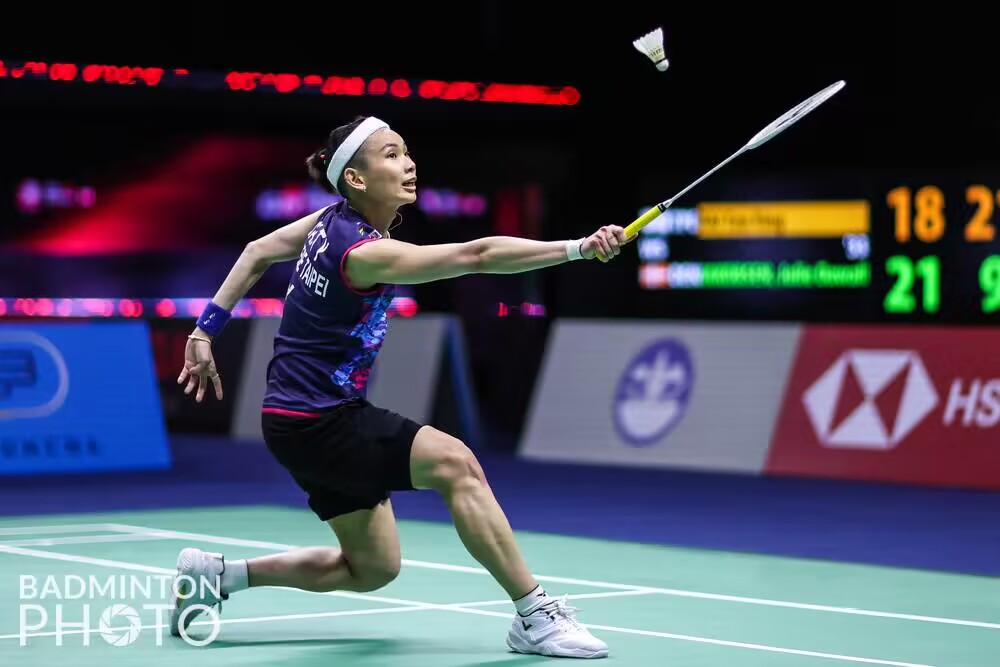
\includegraphics[width=0.9\linewidth]{figure/figure_1.jpg}
% 		\caption{title1}
% 		\label{label1} %文中引用该图片代号
% 	\end{minipage}
% 	%\qquad
% 	\begin{minipage}{0.49\linewidth}
% 		\centering
% 		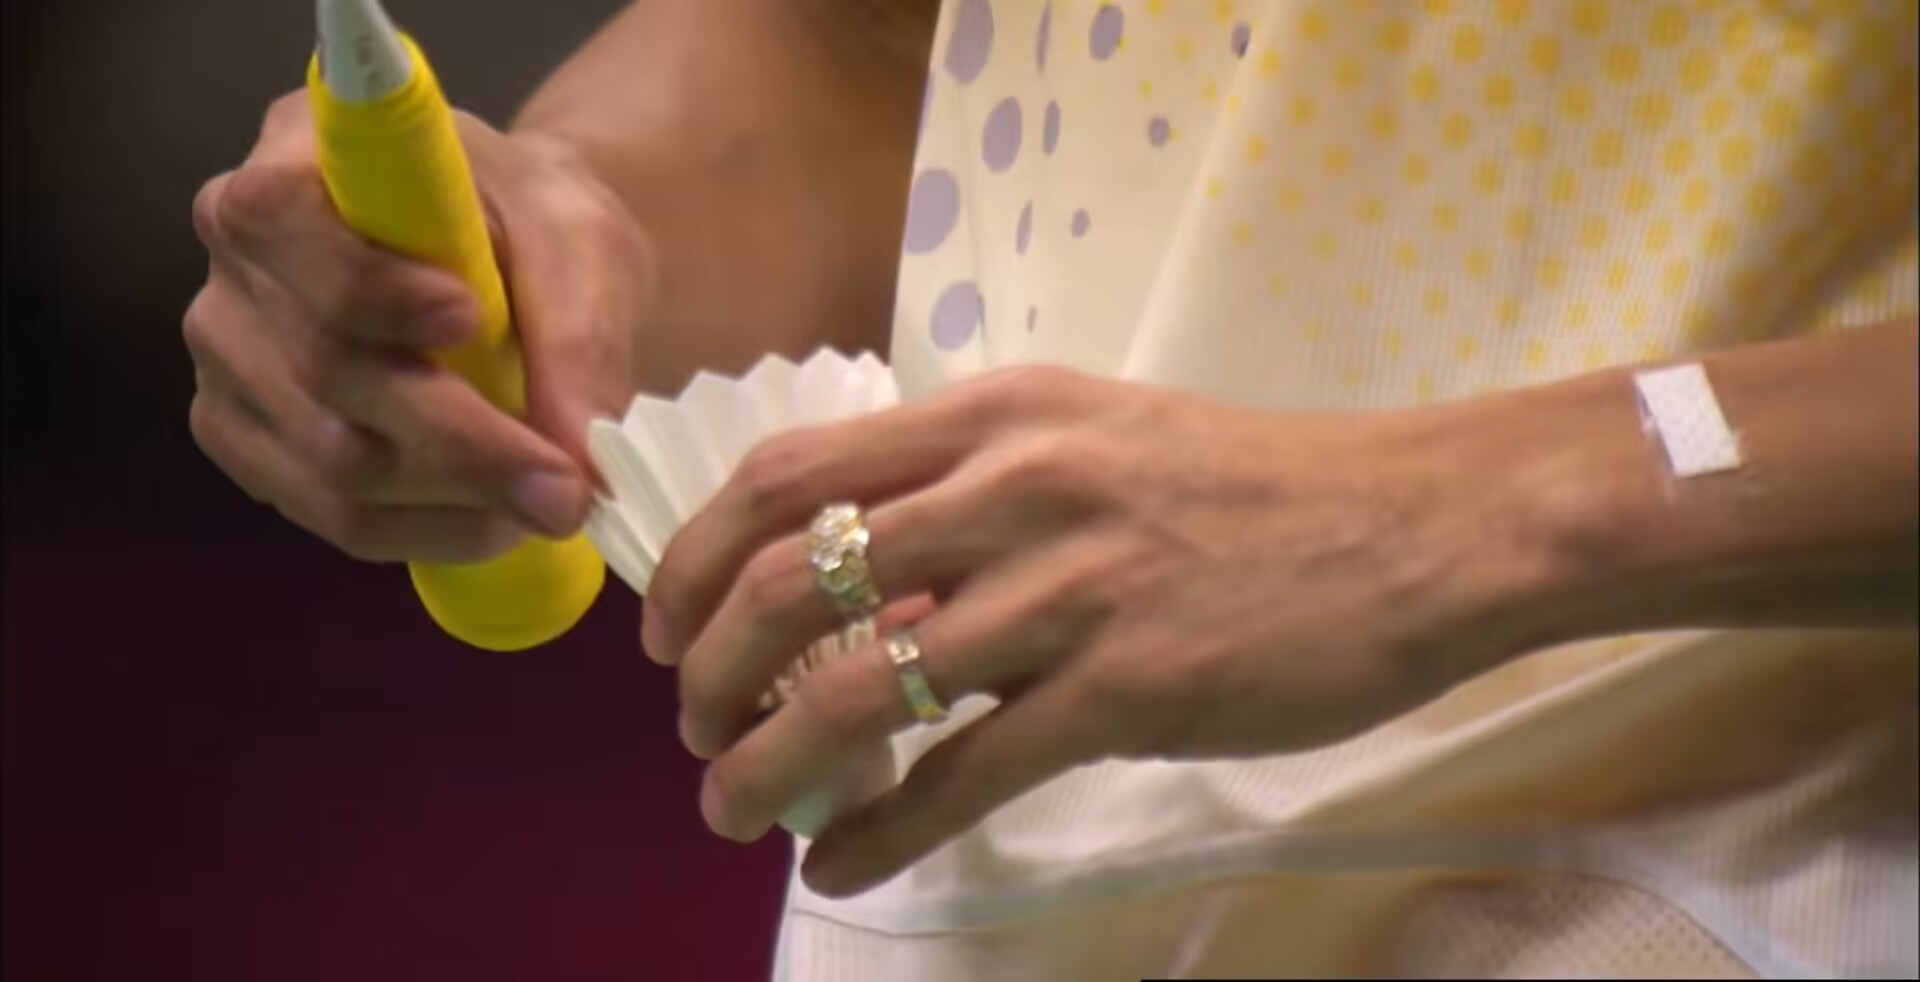
\includegraphics[width=0.9\linewidth]{figure/figure_3.jpg}
% 		\caption{title2}
% 		\label{label2} %文中引用该图片代号
% 	\end{minipage}
% \end{figure}

% 表格加载图片
% \begin{table}[H]
%     \centering % 居中 
%     \caption{模糊控制器-模糊规则表} % caption是图片的标题
%     % 图片文件的相对路径
%     \includegraphics[width=.8\textwidth]{figure/模糊控制器-模糊规则表.png} 
%     \label{tab:模糊控制器-模糊规则表}
% \end{table}

%% 三线表
% \begin{table}[H] % 防止表格乱跑
% \centering % 居中
% \caption{title} % 标题
% \begin{tabular}{cccccc} % 指明列数
% 	\toprule % 顶部粗线
% 	序号 & 姓名 & 性别 & 年龄 & 身高/cm & 体重/kg \\
% 	\midrule % 中间细线
% 	1 & 张三 & M & 16 & 163 & 50 \\ % 每行末尾都要加换行符
% 	2 & 王红 & F & 15 & 159 & 47 \\
% 	3 & 李二 & M & 17 & 165 & 52 \\
% 	\bottomrule % 底部粗线
% \end{tabular}
% \label{tab:模糊控制器-模糊规则表}
% \end{table}


%% 自定义有序列表
% 需要加载enumitem包:\usepackage{enumitem}
% \begin{enumerate}[label=\arabic*、]  % 阿拉伯数字 + '、'
%     \item First step
%     \item Second step
%     \item Third step
% \end{enumerate}

%% 单行公式
% \begin{equation}
%     sin(x) = y
% \label{equa:集总参数钻柱模型} % 公式引用 \ref
% \end{equation}

%% 代码块 
% \begin{lstlisting}
%     hello world
% \end{lstlisting}
%%%%%%%%%%%%%%%%%%%%%%%%%%%%%%%%%%%


% 文档主体
\begin{document}
% 设置正文字体为小四 宋体(封装待完善)
% \setmainfont{Times New Roman}
% \fontsize{12pt}{15pt}\selectfont

% \begin{titlepage}
% % 导入封面
% 
\includepdf[pages={1}]{./cover/cover.pdf}
% \end{titlepage}


% 正文之前不设置页码
% \pagestyle{empty}
% % 中文摘要
% \begin{cnabstract}
% 	这里是摘要这里是摘要这里是摘要这里是摘要这里是摘要这里是摘要这里是摘要这里是摘要这里是摘要这里是摘要这里是摘要这里是摘要这里是摘要这里是摘要这里是摘要这里是摘要这里是摘要这里是摘要这里是摘要这里是摘要
    
%     \vspace{10pt} % 指定行间距
% 	\noindent \textbf{关键词}:关键词1,关键词2,关键词3
% \end{cnabstract}
% \clearpage

% % 生成目录
% \tableofcontents
% \cleardoublepage

% % 页码从正文第一页开始
% \pagestyle{plain}
% \pagenumbering{arabic} % 从这里开始阿拉伯数字页码
% \setcounter{page}{1} % 从1开始页码

% 这里是正文

% % 一级标题
% \section{sec1}
% %% 二级标题
% \subsection{subsec1}
% %%% 三级标题
% \subsubsection{subsubsec1}
% 这里是正文这里是正文这里是正文这里是正文这里是正文这里是正文这里是正文这里是正文这里是正文这里是正文这里是正文这里是正文这里是正文这里是正文这里是正文这里是正文这里是正文这里是正文这里是正文这里是正文这里是正文这里是正文这里是正文这里是正文这里是正文这里是正文这里是正文这里是正文这里是正文这里是正文这里是正文这里是正文这里是正文这里是正文这里是正文这里是正文

% \section{sec2}
% \subsection{subsec2}


% \subsubsection{subsubsec2}




% \begin{thebibliography}{9}
%     \bibitem{texbook}
%     Donald E. Knuth (1986) \emph{The \TeX{} Book}, Addison-Wesley Professional.
    
%     \bibitem{lamport94}
%     Leslie Lamport (1994) \emph{\LaTeX: a document preparation system}, Addison
%     Wesley, Massachusetts, 2nd ed.
% \end{thebibliography}


    



\newpage
\bibliography{ref} % 引用文献的文件名
% 引用方法:\cite{name}
% 将附录添加到目录中
\addcontentsline{toc}{section}{参考文献}


\end{document}
